\documentclass[a4paper,11pt]{article}
\usepackage[T1]{fontenc}
\usepackage[utf8]{inputenc}
\usepackage[a4paper]{geometry}
\geometry{verbose,tmargin=2.5cm,bmargin=2.5cm,lmargin=2.5cm,rmargin=2.5cm}
\pagestyle{Ruled}
\usepackage{array}
\usepackage{verbatim}
\usepackage{prettyref}
\usepackage{booktabs}
\usepackage{textcomp}
\usepackage{url}
\usepackage{amsmath}
\usepackage{chemarr}%flechas para reacciones químicas (SFER.tex)
\usepackage{graphicx}
\usepackage{amssymb}
\usepackage{nomencl}
\usepackage[usenames,dvipsnames]{xcolor}

% the following is useful when we have the old nomencl.sty package
% \providecommand{\printnomenclature}{\printglossary}
% \providecommand{\makenomenclature}{\makeglossary}
\makenomenclature

\usepackage{subfig}
%Configuración de los caption
\PassOptionsToPackage{caption=false}{subfig}%Evita que el paquete subfig lo descabale todo
\captiontitlefont{\itshape}
\captionnamefont{\scshape}
\captionstyle{\centering}
\hangcaption
\usepackage{cancel}
\usepackage{steinmetz}
\usepackage{diffcoeff}
\usepackage{mathtools}

\newtheorem{exerciseT}{Ejemplo}[chapter]

\usepackage[spanish]{babel}
\addto\shorthandsspanish{\spanishdeactivate{~<>}}


\usepackage{siunitx}
\DeclareSIUnit\kWh{kWh}
\DeclareSIUnit{\watthour}{Wh}
\DeclareSIUnit\Wh{Wh}

\sisetup{per-mode=symbol-or-fraction}
%\usepackage{lscape}
\usepackage{mathpazo}%Letra palatino con fuentes para matemáticas
\usepackage{flafter}%obliga a que los flotantes aparezcan después de su referencia
\usepackage{memhfixc}


\raggedbottom
\sloppybottom
\clubpenalty=10000
\widowpenalty=10000

%\raggedbottomsection
\feetbelowfloat


% \usepackage[citestyle=alphabetic, bibstyle=alphabetic, maxbibnames=5,minbibnames=3,
% backend=bibtex, doi=true, url=true]{biblatex}

% \DefineBibliographyStrings{spanish}{%
%   andothers        = {et\addabbrvspace al\adddot},
%   andmore          = {et\addabbrvspace al\adddot},
%   in               = {},
% }

% \let\cite\parencite

% \renewcommand{\bibsection}{%
% 	\chapter*{\bibname}
% 	\bibmark
% 	\phantomsection
% 	\addcontentsline{toc}{chapter}{\bibname}
% 	\prebibhook}
% % \renewcommand{\bbltechreport}{Informe T\'ecnico}

\usepackage{hyperref}


\hypersetup{
    bookmarks=true,         % show bookmarks bar?
    unicode=true,          % non-Latin characters in Acrobat’s bookmarks
    bookmarksnumbered=false,
    bookmarksopen=false,
    breaklinks=true,
    backref=true,
    pdftoolbar=true,        % show Acrobat’s toolbar?
    pdfmenubar=true,        % show Acrobat’s menu?
    pdffitwindow=false,     % window fit to page when opened
    pdfstartview={FitH},    % fits the width of the page to the window
    pdftitle={Teoria de Circuitos},    % title
    pdfauthor={Ana Fernández-Guillamón},     % author
    pdfsubject={ETSIDI},   % subject of the document
    pdfcreator={Overleaf},   % creator of the document
    pdfproducer={LaTeX}, % producer of the document
    pdfnewwindow=true,      % links in new window
    pdfborder={0 0 0},
    colorlinks=true,       % false: boxed links; true: colored links
    linkcolor=Brown,          % color of internal links
    citecolor=BrickRed,        % color of links to bibliography
    filecolor=black,      % color of file links
    urlcolor=Blue           % color of external links 
}

\addto\captionsspanish{%
\def\tablename{Tabla}%
\def\listtablename{\'Indice de tablas}}


%\spanishdecimal{.} %Para que no lo sustituya automáticamente por comas
\def\nompreamble{\addcontentsline{toc}{chapter}{\nomname}\markboth{\nomname}{\nomname}}

%Configuración de MEMOIR
%%Pone la fecha en SMALL CAPS y hacia la derecha
%%pagina 60 de memman.pdf
\pretitle{
\vfill
\centering \bfseries \scshape \HUGE \color{BrickRed}
\posttitle{\par}
}

\preauthor{
\vfill
\centering
\large \scshape
\postauthor{
\par }
}

\predate{\vfill \begin{flushright}\large\scshape}
\postdate{\par\end{flushright}\vfill}


\setsecnumdepth{subsection}


% \definecolor{ared}{rgb}{.647,.129,.149}
% \renewcommand{\colorchapnum}{\color{ared}}
% \renewcommand{\colorchaptitle}{\color{ared}}
% \chapterstyle{pedersen}
\chapterstyle{ger}

\setlength{\afterchapskip}{35pt}
\maxtocdepth{section}

%\setcounter{topnumber}{3}
%\setcounter{bottomnumber}{2}
%\setcounter{totalnumber}{4}
\renewcommand{\topfraction}{0.85}
\renewcommand{\bottomfraction}{0.5}
\renewcommand{\textfraction}{0.15}
\renewcommand{\floatpagefraction}{0.7}


\usepackage{float}

\RequirePackage[framemethod=default]{mdframed} % Required for creating the theorem, definition, exercise and corollary boxes

% Exercise box	  
\newmdenv[skipabove=7pt,
skipbelow=7pt,
rightline=false,
leftline=false,
topline=false,
bottomline=false,
backgroundcolor=BrickRed!10,
linecolor=BrickRed,
innerleftmargin=5pt,
innerrightmargin=5pt,
innertopmargin=5pt,
innerbottommargin=5pt,
leftmargin=0cm,
rightmargin=0cm,
linewidth=4pt]{eBox}

\newenvironment{example}{\begin{eBox}\begin{exerciseT}}{\hfill{\color{BrickRed}\tiny\ensuremath{\blacksquare}}\end{exerciseT}\end{eBox}}	


\renewcommand{\textfloatsep}{10pt}%Espacio entre el flotante y el texto

\usepackage{tikz}
\newenvironment{remark}{\par\vspace{10pt}\small % Vertical white space above the remark and smaller font size
\begin{list}{}{
\leftmargin=35pt % Indentation on the left
\rightmargin=25pt}\item\ignorespaces % Indentation on the right
\makebox[-2.5pt]{\begin{tikzpicture}[overlay]
\node[draw=BrickRed!60,line width=1pt,circle,fill=BrickRed!25,font=\sffamily\bfseries,inner sep=2pt,outer sep=0pt] at (-15pt,0pt){\textcolor{BrickRed}{N}};\end{tikzpicture}} % Orange R in a circle
\advance\baselineskip -1pt}{\end{list}\vskip5pt} % Tighter line spacing and white space after remark 

\title{Problemas de corriente alterna trifásica}

\date{}

\author{ETSIDI}

%%%%% EMPIEZA EL DOCUMENTO

\begin{document}

\maketitle

%%%%% PROBLEMAS

\section{} 
\begin{wrapfigure}[6]{r}{0.35\textwidth}
		\centering
		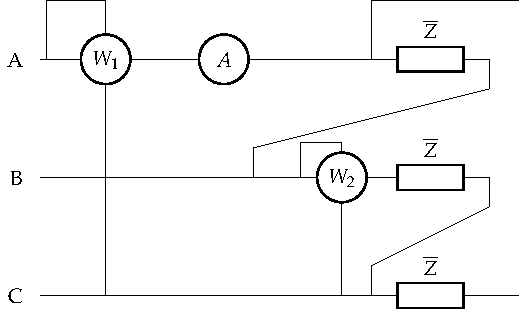
\includegraphics[width=0.35\textwidth]{figuras/ej1_CAtrif.pdf}
	\end{wrapfigure}
En el sistema de la figura de secuencia de fases directa y frecuencia $f=\SI{60}{\hertz}$, se dispone de un receptor equilibrado con una potencia total $P_T=\SI{51984}{\watt}$ factor de potencia de $0.6$ en retraso. Sabiendo que el amperímetro marca $\SI[parse-numbers=false]{76\sqrt{3}}{\ampere}$, determinar:
\begin{enumerate}
    \item Medida delos vatímetros 1 y 2.
    \item Valor de la impedancia $\overline{Z}$ en forma módulo-argumento.
    \item Valor de la capacidad mínima para mejorar el factor de potencia a $0.95$ en retraso.
    \item Valor de la impedancia equivalente en estrella.
\end{enumerate}

\subsection{}

%% SOLUCION
Para solucionar las preguntas en este problema, antes de calcular nada, podemos extraer la siguiente información del enunciado:
\begin{itemize} % para incluir viñetas
    \item Se tiene una sola carga trifásica equilibrada de valor $Z$ y con $\cos{\phi}=0,6\rightarrow \SI{53.13}{\degree}$ en retraso. Esto significa que la impedancia $\overline{Z}$ es de carácter inductivo y su potencia reactiva será positiva.
    \item 	Se tiene una secuencia de fases directa ABC. Esto significa que el sistema de alimentación tiene las siguientes tensiones de línea: $\overline{U_{AB}}=\SI[parse-numbers=false]{U_{AB}\phase{\SI{120}{\degree}}}{\volt}$, $\overline{U_{BC}}=\SI[parse-numbers=false]{U_{BC}\phase{\SI{0}{\degree}}}{\volt}$ y $\overline{U_{CA}}=\SI[parse-numbers=false]{U_{CA}\phase{\SI{-120}{\degree}}}{\volt}$. Así pues, las tensiones de fase son: $\overline{U_{A}}=\SI[parse-numbers=false]{U_{A}\phase{\SI{90}{\degree}}}{\volt}$, $\overline{U_{B}}=\SI[parse-numbers=false]{U_{B}\phase{\SI{-30}{\degree}}}{\volt}$ y $\overline{U_{C}}=\SI[parse-numbers=false]{U_{C}\phase{\SI{-150}{\degree}}}{\volt}$.
    \item Anotamos la frecuencia de red de valor $\SI{60}{\hertz}$ por si hemos de calcular alguna reactancia inductiva y/o capacitiva.
    \item La potencia activa total que demanda el triángulo de impedancia $\overline{Z}$ es de valor $P_T=\SI{51984}{\watt}$. De este valor, sacamos como conclusión que cada impedancia $\overline{Z}$ del triángulo consume un tercio de dicha potencia activa al ser un receptor equilibrado.
    \item El vatímetro $W_2$ está conectado midiendo la intensidad $\overline{I_{BC}}$ y la tensión $\overline{U_{BC}}$, es decir, nos da el valor de la potencia activa que disipa la fase BC del triángulo, cuyo valor ya sabemos que es:
    \[
        W_2=\dfrac{P_T}{3}=\dfrac{51984}{3}=\SI{17328}{\watt}
    \]
    \item El amperímetro dispuesto en la línea A mide el valor eficaz de $\SI[parse-numbers=false]{76\sqrt{3}}{\ampere}$. Esto significa que, al tener un receptor equilibrado conectado en triángulo, las intensidades por las otras dos líneas B y C tienen el mismo valor de intensidad de valor eficaz de $\SI[parse-numbers=false]{76\sqrt{3}}{\ampere}$.
    \item También, al ser un receptor equilibrado conectado en triángulo, las intensidades $\overline{I_{AB}}$, $\overline{I_{BC}}$ e $\overline{I_{CA}}$ que circulan dentro del triángulo, toman por valor eficaz:
    \[
    \dfrac{76\sqrt{3}}{\sqrt{3}}=\SI{76}{\ampere}
    \]
    \item 	Los argumentos de las intensidades dentro de triángulo se pueden obtener del propio enunciado. Cada intensidad $\overline{I_{AB}}$, $\overline{I_{BC}}$ e $\overline{I_{CA}}$ retrasa $\SI{53,13}{\degree}$ a las tensiones $\overline{U_{AB}}$, $\overline{U_{BC}}$ y $\overline{U_{CA}}$ correspondientes, es decir, la intensidad $\overline{I_{AB}}$ tiene un argumento de valor $120-53,13=\SI{66,87}{\degree}$, la intensidad $\overline{I_{BC}}$ tiene un argumento de valor $0-53,13=\SI{-53,13}{\degree}$ y la intensidad $\overline{I_{CA}}$ tiene un argumento de valor $-120-53,13=\SI{-153,13}{\degree}$.
    \item 	Los argumentos de las intensidades de línea también se pueden obtener del propio enunciado. Cada intensidad $\overline{I_A}$, $\overline{I_B}$ e $\overline{I_C}$ retrasa $\SI{53,13}{\degree}$ a las tensiones del sistema de alimentación $\overline{U_A}$, $\overline{U_B}$ y $\overline{U_C}$ correspondientes, es decir, la intensidad $\overline{I_A}$ tiene un argumento de valor $90-53,13=\SI{36,87}{\degree}$, la intensidad $\overline{I_B}$ tiene un argumento de valor $-30-53,13=\SI{-83,13}{\degree}$ y la intensidad $\overline{I_C}$ tiene un argumento de valor $-150-53,13=\SI{-203,13}{\degree}$.
\end{itemize}

Tras estas consideraciones, se pueden iniciar los cálculos necesarios para responder a las preguntas del problema:
\begin{enumerate}
    \item 	Medida de los vatímetros 1 y 2.
    
La lectura del vatímetro 1, según está conectado, es la siguiente:
\[
[W_1]=\overline{U_{AC}}\cdot \overline{I _A}=U_{AC}\cdot I_A\cdot \cos(\langle \overline{U_{AC}}, \overline{I_A} \rangle)
\]

Se desconoce el módulo de la tensión $\overline{U_{AC}}$. Se calcula a partir del vatímetro 2 cuya lectura es de $[W_2]=\SI{17328}{\watt}$:
\[
[W_2]=\overline{U_{BC}}\cdot \overline{I_{BC}}=U_{BC}\cdot I_{BC}\cdot \cos(\langle \overline{U_{BC}}; \overline{I_{BC}}\rangle);\; 17328=U_{BC}\cdot 76\cdot 0.6\Rightarrow U_{BC}=\SI{380}{\volt}
\]
Por tanto, al ser un sistema equilibrado ($U_{AB}=U_{BC}=U_{CA}$), y sabiendo que $\overline{U_{AC}}=-\overline{U_{CA}}=U_{CA}\phase{-120+180}=\SI[parse-numbers=false]{380\phase{\SI{60}{\degree}}}{\volt}$, la lectura del vatímetro 1:
\[
[W_1]=\overline{U_{AC}}\cdot \overline{I_A}=U_{AC}\cdot I_A\cdot \cos(\langle \overline{U_{AC}}, \overline{I_A} \rangle)=380\cdot 76\sqrt{3}\cdot \cos(\langle60;36.87\rangle)=\SI{46001}{\watt}
\]

\item Valor de la impedancia $\overline{Z}$ en forma módulo-argumento.

Al conocer ya el valor de la tensión a la que está alimentada y la intensidad que circula por ella, se obtiene su valor fácilmente a partir de la ley de Ohm:
\[
\overline{Z}=\dfrac{\overline{U_{AB}}}{\overline{I_{AB}}}=\dfrac{380\phase{120}}{76\phase{66.87}}=\SI[parse-numbers=false]{5\phase{\SI{53.13}{\degree}}}{\ohm}
\]

\item Valor de la capacidad mínima para mejorar el factor de potencia a $0.95$ en retraso.




    \item Valor de la impedancia equivalente en estrella.


\end{enumerate}

\section{} 
% poner aqui el ENUNCIADO DEL PROBLEMA

\subsection{}

% poner aqui la SOLUCION DEL PROBLEMA	


\newpage{}


\end{document}